\documentclass[]{beamer}
\setbeamertemplate{sidebar right}{}
\setbeamertemplate{footline}{
\hfill\usebeamertemplate***{navigation symbols}
\hspace{1cm}\insertframenumber}

\title{Robust Methods for Optical \\ Interferometry
    Images}
\subtitle[short version]{Ph.D Thesis}
\author{M. en C. Orlando Miguel Medina C\'azares}
\date{23 de Noviembre del 2015}
\institute[CIO]{Centro de Investigaciones en \'Optica}
\logo{
\includegraphics[scale=0.30]{Images/cio_logo.png}}

\begin{document}
%%%%%%%%%%%%%%%%%%%%%%%%%%%% 
\begin{frame}[plain]
  \maketitle
  \footnotesize{
    Asesor: Dr. Julio Estrada Rico. \\
    Co-Asesor: Dr Manuel Servin Guirado.
  }
\end{frame}
%%%%%%%%%%%%%%%%%%%%%%%%%%%%
%\begin{frame}
%\frametitle{Outline}
%\tableofcontents[part=1,pausesections]
%\end{frame}
%%%%%%%%%%%%%%%%%%%%%%%%%%%% 2
\begin{frame}{Algoritos de Cuadratura}
  Patr\'on de franjas:
  \begin{equation}
    I(x,y)=a(x,y)+b(x,y)cos[\phi(x,y)]
  \end{equation}
  \begin{center}
    \pause 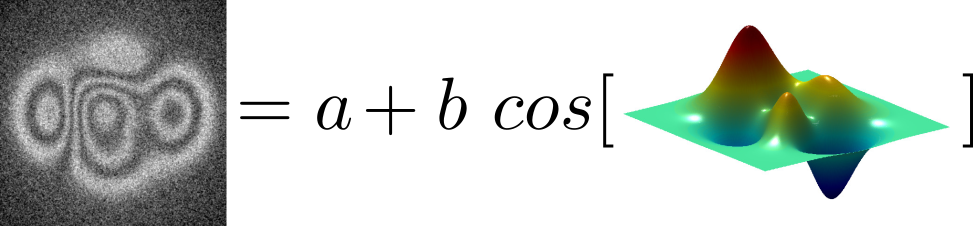
\includegraphics[scale=0.4]{Images/Interferogram.png}
  \end{center}
\end{frame}
%%%%%%%%%%%%%%%%%%%%%%%%%%%% 3
\begin{frame}{Algoritos de Cuadratura}
  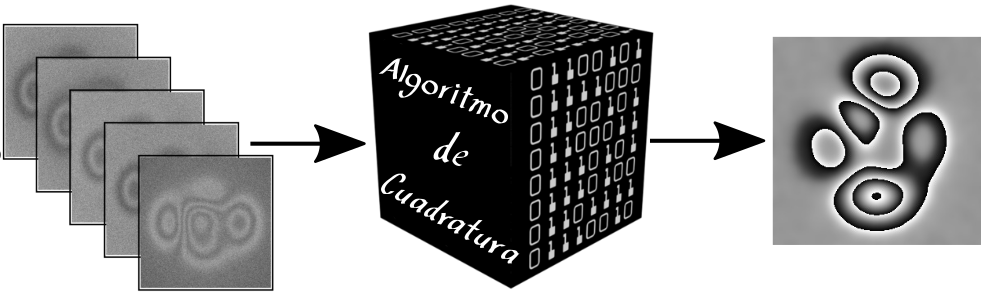
\includegraphics[scale=0.4]{Images/QuadratureFiltersScheme2.png}
\end{frame}
%%%%%%%%%%%%%%%%%%%%%%%%%%%% 4
\begin{frame}{Algoritos de Cuadratura}
\begin{center}

    \begin{eqnarray}
                      \mathcal{F}[I(x,y)] & = & I(\omega) \nonumber \\
                                                  & = & a\delta(\omega)+
                      \frac{b}{2}e^{-i \phi} \delta(\omega-\omega_0) +
                      \frac{b}{2} e^{i \phi} \delta(\omega+\omega_0)
    \end{eqnarray}
    \pause 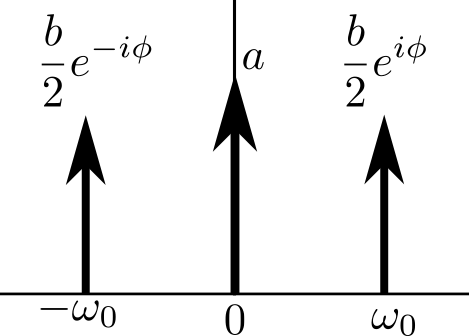
\includegraphics[scale=0.6]{Images/FourierDomine1.png}

\end{center}
\end{frame}
%%%%%%%%%%%%%%%%%%%%%%%%%%%% 5
\begin{frame}{Algoritos de Cuadratura}
\begin{center}

  \begin{equation}
            H(-\omega_0) =H(0) = 0, H(\omega_0) \neq 0
  \end{equation}
  \pause 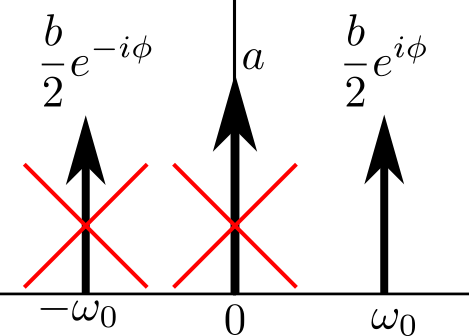
\includegraphics[scale=0.6]{Images/FourierDomine2.png} 

\end{center}
\end{frame}
%%%%%%%%%%%%%%%%%%%%%%%%%%%% 6
\begin{frame}{Algoritos de Cuadratura}
\begin{center}

    \begin{equation}
             I(\omega) H(\omega) = \frac{b}{2}exp[i \phi]
     \end{equation}
     \pause 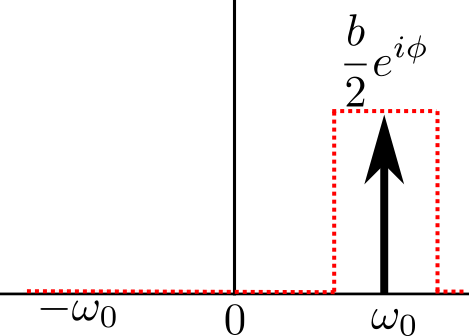
\includegraphics[scale=0.6]{Images/FourierDomine3.png}

  \end{center}
\end{frame}
%%%%%%%%%%%%%%%%%%%%%%%%%%%% 7
\begin{frame}{Algoritmos de Cuadratura}
\begin{center}

  \begin{equation}
    \hat \phi=atan\bigg[ \frac{ Im\{\frac{b}{2}exp[i \phi]\} }{
      Re\{\frac{b}{2}exp[i \phi]\} } \bigg] = atan\bigg[  \frac{sin[\phi]}{cos[\phi]}\bigg]
  \end{equation}
  \pause 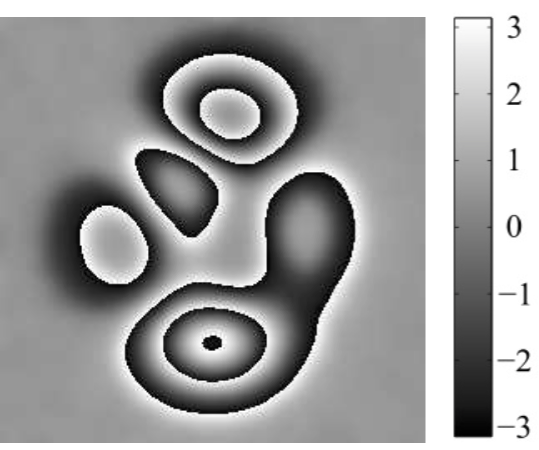
\includegraphics[scale=0.6]{Images/wPhase.png}

\end{center}
\end{frame}
%%%%%%%%%%%%%%%%%%%%%%%%%%%% 8
\begin{frame}{Filtros Regularizados}
\begin{center}

\begin{eqnarray}
  U[f(x,y)] &=&\iint_{(x,y) \in S} \Bigg\{ [f(x,y)-I(x,y)]^2 +  \nonumber \\
     & & \eta \bigg[  \frac{\partial f(x,y)}{\partial x} \bigg]^2 +
            \eta \bigg[  \frac{\partial f(x,y)}{\partial y} \bigg]^2 
     \Bigg\} dx dy
\end{eqnarray}
\pause 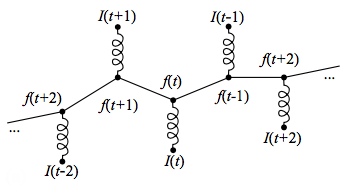
\includegraphics[scale=0.6]{Images/RegularizadosResorte.png}

\end{center}
\end{frame}
%%%%%%%%%%%%%%%%%%%%%%%%%%%% 9
\begin{frame}{Filtros Regularizados}
\begin{center}

\begin{eqnarray}
  U[f(x,y)] &=&\iint_{(x,y) \in S} \Bigg\{ [f(x,y)-I(x,y)]^2 + 
     \eta \bigg[  \frac{\partial ^2 f(x,y)}{\partial x^2} \bigg]^2 +
                \nonumber \\
      & &\eta \bigg[  \frac{\partial ^2 f(x,y)}{\partial y^2} \bigg]^2 +
     \eta \bigg[  \frac{\partial ^2 f(x,y)}{\partial x \partial y} \bigg]^2
     \Bigg\} dx dy
\end{eqnarray}
\pause 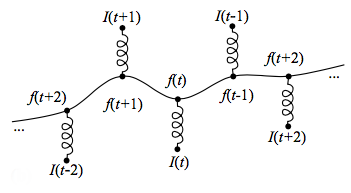
\includegraphics[scale=0.6]{Images/RegularizadosPlaca.png}

\end{center}
\end{frame}
%%%%%%%%%%%%%%%%%%%%%%%%%%%% 10
\begin{frame}{Filtros Regularizados}
%\begin{center}

Funcional:
\begin{equation}
  U[f(x,y)]= \sum_{(x,y) \in S} \Big\{  [ f(x,y)-I(x,y) ]^2 + \eta R[f(x,y)] \Big\} 
\end{equation}

Regularizador Resorte:
\begin{equation}
  \pause R_r [f(x,y)] = [f(x,y)-f(x-1,y)]^2 + [f(x,y)-f(x,y-1)]^2 
\end{equation}

Regularizador Placa:
\begin{eqnarray}
  \pause R_p [f(x,y)] & = & [f(x+1,y)-2f(x,y)-f(x-1,y)]^2 \nonumber \\
  & & + [f(x,y+1)-2f(x,y)-f(x,y-1)]^2 \nonumber \\
  & & + [ f(x+1,y+1)-f(x-1,y-1) \nonumber \\ 
  & & + f(x-1,y+1)-f(x+1,y-1) ]^2
\end{eqnarray}

%\end{center}
\end{frame}
%%%%%%%%%%%%%%%%%%%%%%%%%%%% 11
\begin{frame}{Filtros Regularizados}
\begin{center}

Resorte:\\
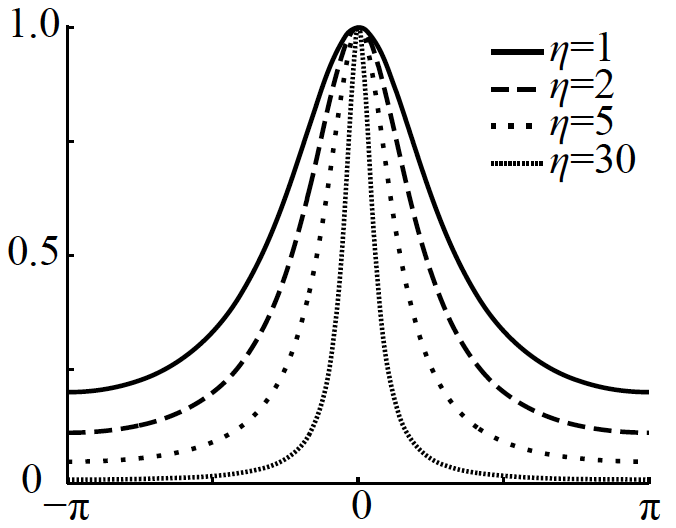
\includegraphics[scale=0.45]{Images/FrecuenciaResorte.png}
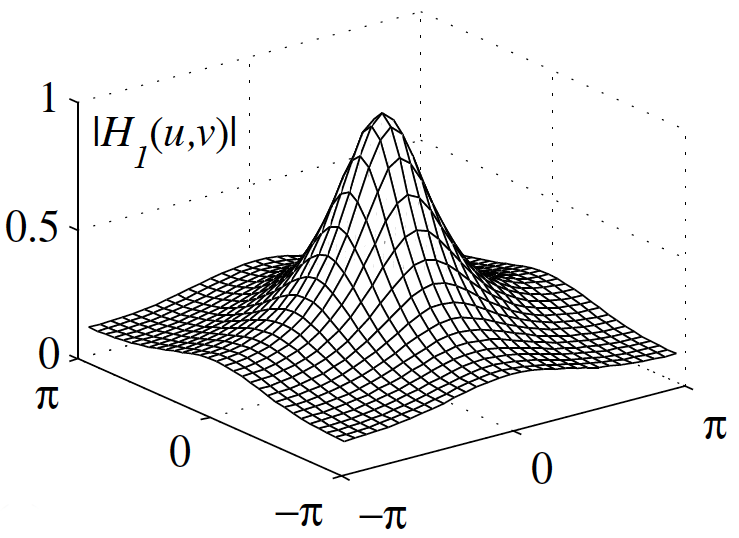
\includegraphics[scale=0.45]{Images/FrecuenciaResorte3D.png}

\end{center}
\end{frame}
%%%%%%%%%%%%%%%%%%%%%%%%%%%% 12
\begin{frame}{Filtros Regularizados}
\begin{center}

Placa:\\
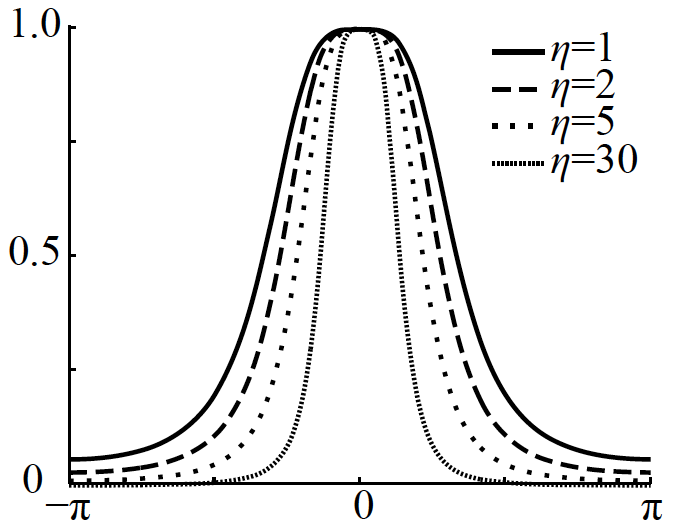
\includegraphics[scale=0.45]{Images/FrecuenciaPlaca.png}
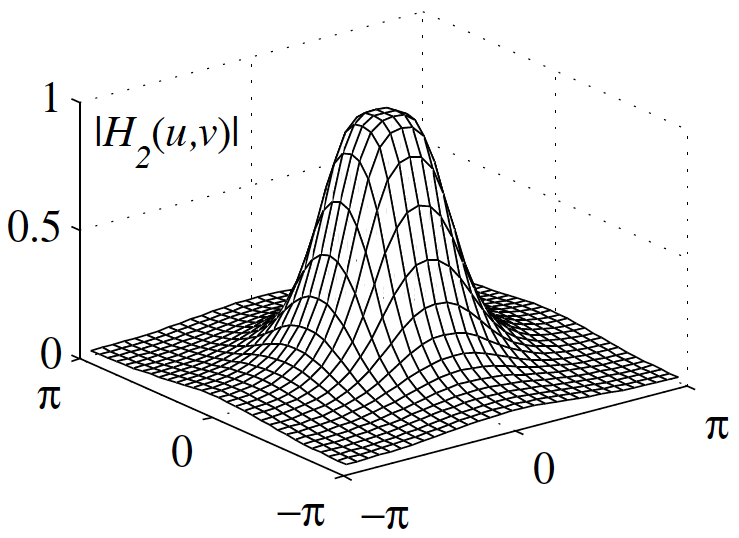
\includegraphics[scale=0.45]{Images/FrecuenciaPlaca3D.png}

\end{center}
\end{frame}
%%%%%%%%%%%%%%%%%%%%%%%%%%%% 13
\begin{frame}{M\'inimos Cuadrados Regularizados}
\begin{center}

\begin{eqnarray}
  I(x,y,k) &=& a(x,y) + b(x,y)\cos[\phi(x,y) +\alpha k] \nonumber \\
  &=& a(x,y) + C(x,y)\cos[\alpha k] - S(x,y)\sin[\alpha k]
\end{eqnarray}
donde:\\
$C(x,y)=b(x,y)\cos[\phi(x,y)]$ \\ 
$S(x,y)=b(x,y)\sin[\phi(x,y)]$\\


\end{center}
\end{frame}
%%%%%%%%%%%%%%%%%%%%%%%%%%%% 14
\begin{frame}{M\'inimos Cuadrados Regularizados}

Funcional de m\'inimos cuadrados:
\begin{center}
\begin{align}
  U[a,C,S]= \sum_{k=0}^{N-1}\left[a + C \cos(\alpha k)\right.
  -\left. S \sin(\alpha k)-I(k) \right]^2
\end{align}

\pause
\scriptsize{
\begin{multline*}
\left(\begin{array}{c}
a(x,y)\\
C(x,y)\\
S(x,y)
\end{array}\right) = \\
\left(\begin{array}{ccc}
K & \sum c_{k}(x,y) & \sum s_{k}(x,y)\\
\sum c_{k}(x,y) & \sum c_{k}(x,y)^{2} & \sum c_{k}(x,y)s_{k}(x,y)\\
\sum s_{k}(x,y) & \sum c_{k}(x,y)s_{k}(x,y) & \sum s_{k}(x,y)^{2}
\end{array}\right)^{-1}
\left(\begin{array}{c}
\sum I_{k}(x,y)\\
\sum I_{k}(x,y)C_{k}(x,y)\\
\sum I_{k}(x,y)S_{k}(x,y)
\end{array}\right)
\end{multline*}
}


\end{center}
\end{frame}
%%%%%%%%%%%%%%%%%%%%%%%%%%%% 15
\begin{frame}{M\'inimos Cuadrados Regularizados}
\begin{center}

  \begin{equation}
     \phi=atan\bigg[ \frac{S(x,y)}{C(x,y)} \bigg] = atan\bigg[  \frac{sin[\phi(x,y)]}{cos[\phi(x,y)]}\bigg]
  \end{equation}
\pause 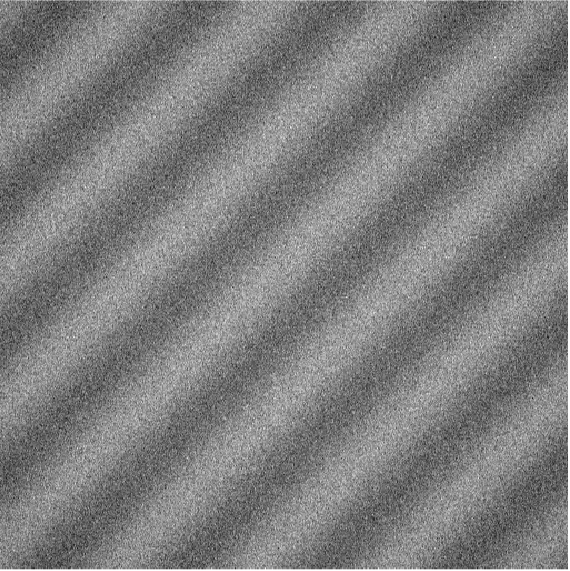
\includegraphics[scale=0.25]{Images/InterferogramLS.png} \quad \quad
\pause 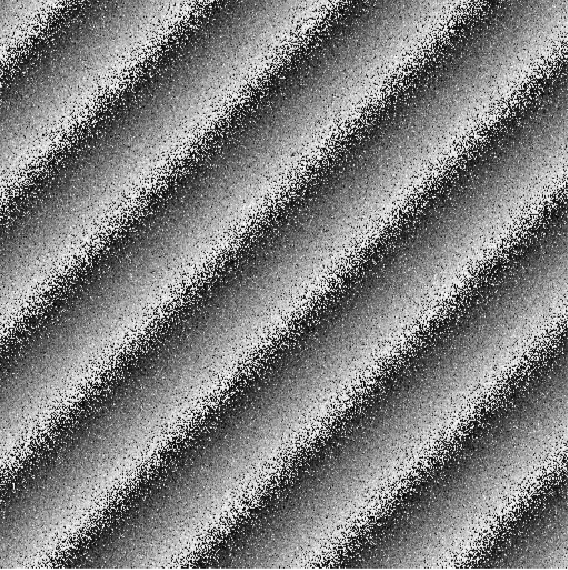
\includegraphics[scale=0.25]{Images/FaseMinCua.png}

\end{center}
\end{frame}
%%%%%%%%%%%%%%%%%%%%%%%%%%%% 16
\begin{frame}{M\'inimos Cuadrados Regularizados}

Funcional de m\'inimos cuadrados regularizados:
\begin{center}
\begin{small}
\begin{align}
  U(\bf{a,C,S})=\nonumber\\
  &\sum_{k=0}^{N-1} \sum_{x,y\in L} \left[a + 
  C\cos(\alpha k)\right.
  -\left. S\sin(\alpha k)-I_k \right]^2 M_{x,y}\nonumber \\
  &+\lambda\sum_{x,y\in L}
  \left[(C_{x,y}-C_{x-1,y})^2+(S_{x,y}-S_{x,y-1})^2\right]M_{x,y}
  \nonumber\\
  &+\mu\sum_{x,y\in L}(a_{x,y}-a_{x-1,y})^2 M_{x,y}
  \label{eq:psi regularized}
\end{align}
\end{small}


\end{center}
\end{frame}
%%%%%%%%%%%%%%%%%%%%%%%%%%%% 17
\begin{frame}{M\'inimos Cuadrados Regularizados}

Resultado usando m\'inimos cuadrados regularizado
\begin{center}
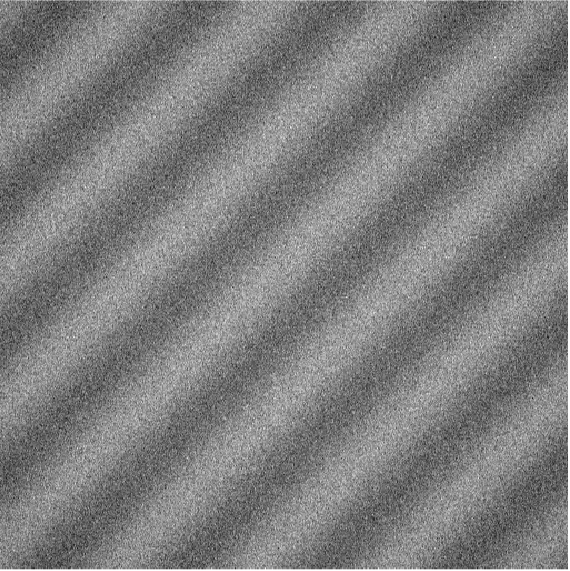
\includegraphics[scale=0.32]{Images/InterferogramLS.png} \quad \quad
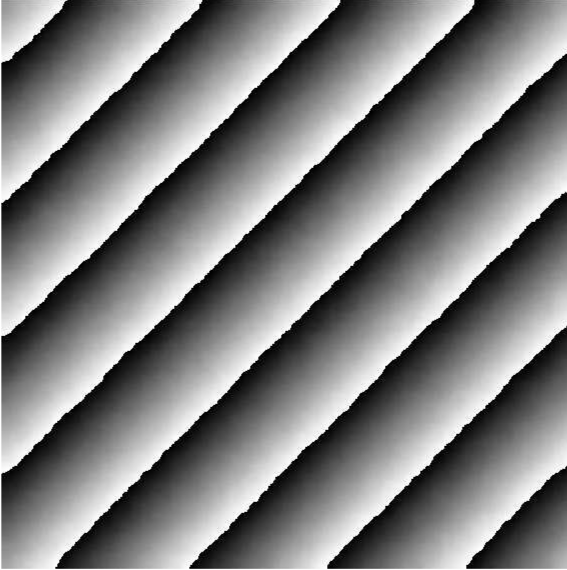
\includegraphics[scale=0.32]{Images/FaseMinCuaReg.png}

\end{center}
\end{frame}
%%%%%%%%%%%%%%%%%%%%%%%%%%%% 18
\begin{frame}{M\'inimos Cuadrados Regularizados}
Comparaci\'on de resultados experimentales

\begin{center}
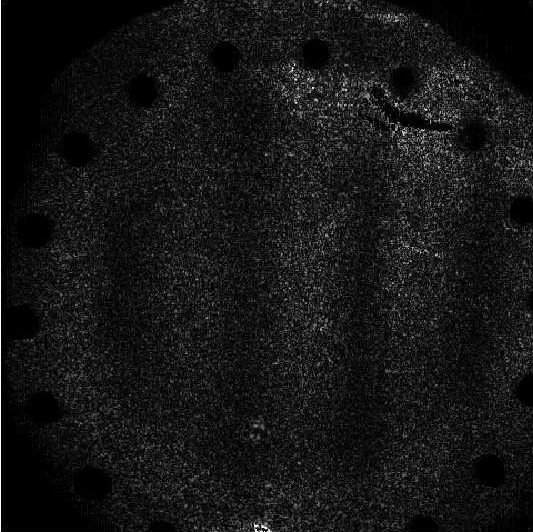
\includegraphics[scale=0.27]{Images/InterferogramLS-exp.png}\\
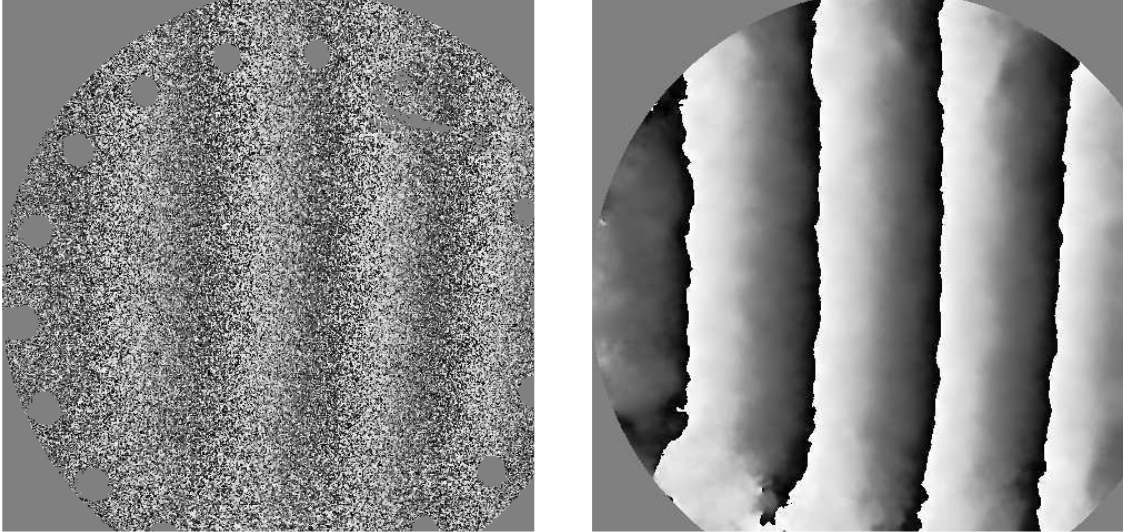
\includegraphics[scale=0.29]{Images/LS-Regularized-exp.png}

\end{center}
\end{frame}
%%%%%%%%%%%%%%%%%%%%%%%%%%%% 19
\begin{frame}{M\'inimos Cuadrados Regularizados}

Conclusiones:
\begin{itemize}
     \item Incorporaci\'on de informaci\'on adyacente.
     \pause \item Interpolaci\'on de peque\~nos espacios vacios (si as\'i se desea).
     \pause \item Recobra una fase limpia de ruido.
\end{itemize}

\end{frame}
%%%%%%%%%%%%%%%%%%%%%%%%%%%% 20
\begin{frame}{Algoritmo auto-entonable para PSI}
Funcional de energ\'ia:
\begin{center}

\begin{eqnarray}
 U(\bf{f,\alpha}) & = &\sum_{k=0}^{N-1}
\sum_{(x,y)}[\frac{1}{2}[f(x,y)e^{i\alpha_{k}}+f^{*}(x,y)e^{-i\alpha_{k}}]-I_{k}
^{'}(x,y)]^{2}\label{eq:U}\nonumber \\
 &  & +\lambda\sum_{(x,y)}[||D_{x}[f(x,y)]||^{2}+||D_{y}[f(x,y)]||^{2}] 
\end{eqnarray}
Donde $f(x,y)=e^{i\phi(x,y)}=cos[\phi(x,y)]+i sin[\phi(x,y)]$

\end{center}
\end{frame}
%%%%%%%%%%%%%%%%%%%%%%%%%%%% 21
\begin{frame}{Algoritmo auto-entonable para PSI}
Remover DC del patr\'on de franjas:
\begin{center}

\begin{equation}
I_{k}^{'}(x,y)=b^{'}(x,y)cos(\phi(x,y)+\alpha_{k}),\: k=0,1,2,...,N-1.
\end{equation}

\begin{equation}
I_{k}^{'}(x,y)=I_{k}(x,y)-[I_{k}*h](x,y),\; k=0,1,2,...,N-1.
\end{equation}
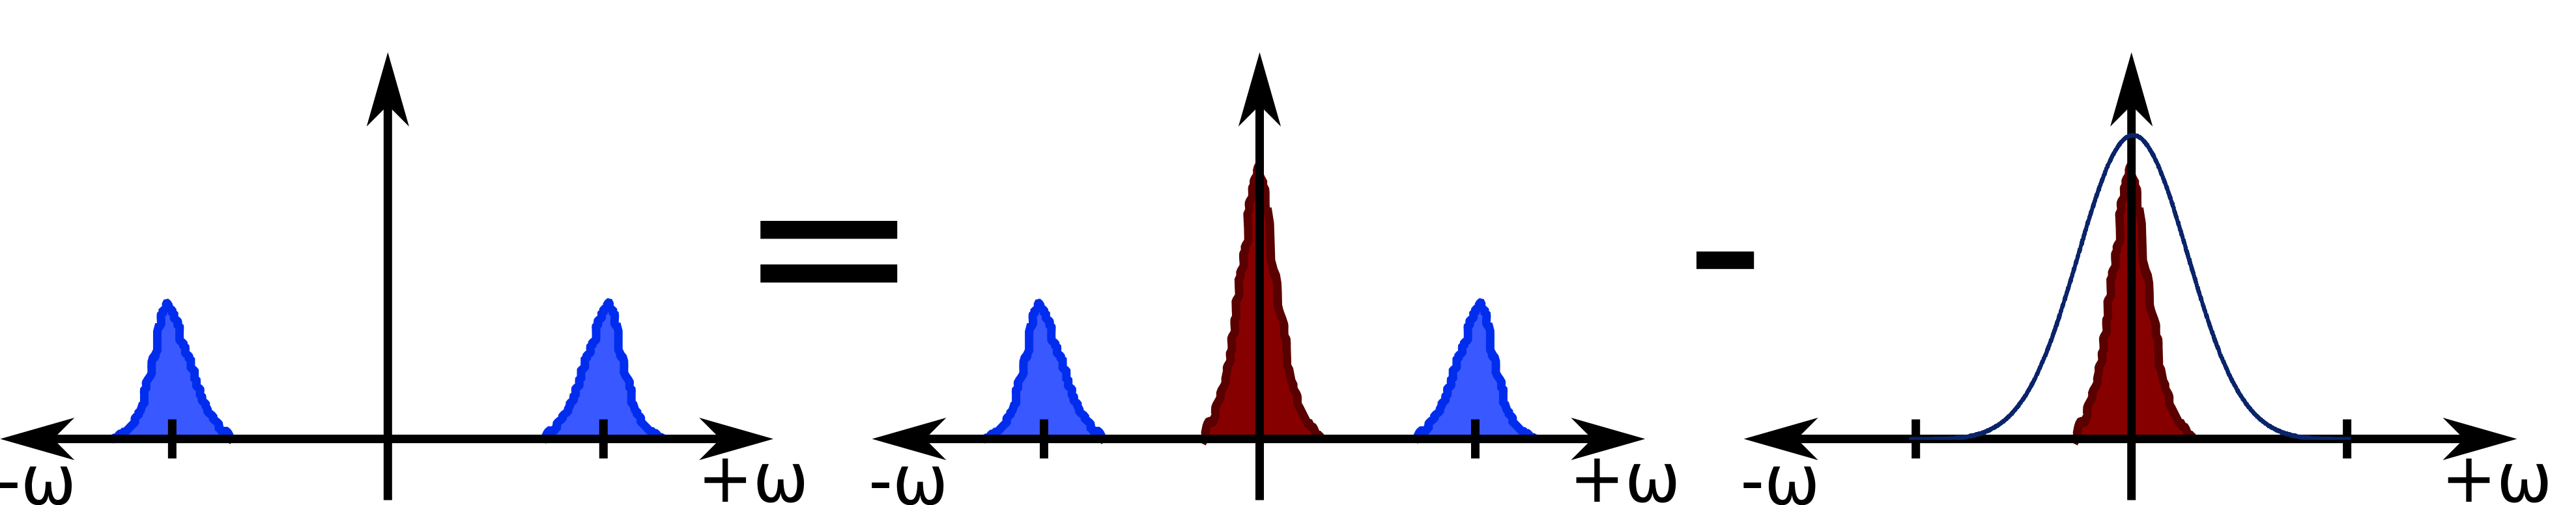
\includegraphics[scale=0.1]{Images/QuitarDC.png}


\end{center}
\end{frame}
%%%%%%%%%%%%%%%%%%%%%%%%%%%% 22
\begin{frame}{Algoritmo auto-entonable para PSI}

Operadores $D_x[]$ y $D_y[]$ toman la primera diferencia:
\begin{center}

\begin{equation}
D_{x}[f(x,y)]=f(x,y)-f(x-1,y)+f(x,y)-f(x+1,y),
\end{equation}
\begin{equation}
D_{y}[f(x,y)]=f(x,y)-f(x,y-1)+f(x,y)-f(x,y+1).
\end{equation}

\end{center}
\end{frame}
%%%%%%%%%%%%%%%%%%%%%%%%%%%% 23
\begin{frame}{Algoritmo auto-entonable para PSI}

Para resolver el funcional separamos el problema en dos.
\begin{itemize}
  
  \pause \item Parte lineal: \\
  \begin{equation}  
    \frac{\partial U}{\partial cos(\phi) }=0,
  \end{equation}
  \begin{equation}  
    \frac{\partial U}{\partial sin(\phi) }=0.
  \end{equation}
  
  \pause \item Parte no lineal:\\
  \begin{equation}  
    \frac{\partial U}{\partial \alpha_k }=0,
  \end{equation}

\end{itemize}

\end{frame}
%%%%%%%%%%%%%%%%%%%%%%%%%%%% 24
\begin{frame}{Algoritmo auto-entonable para PSI}

Fase recobrada:
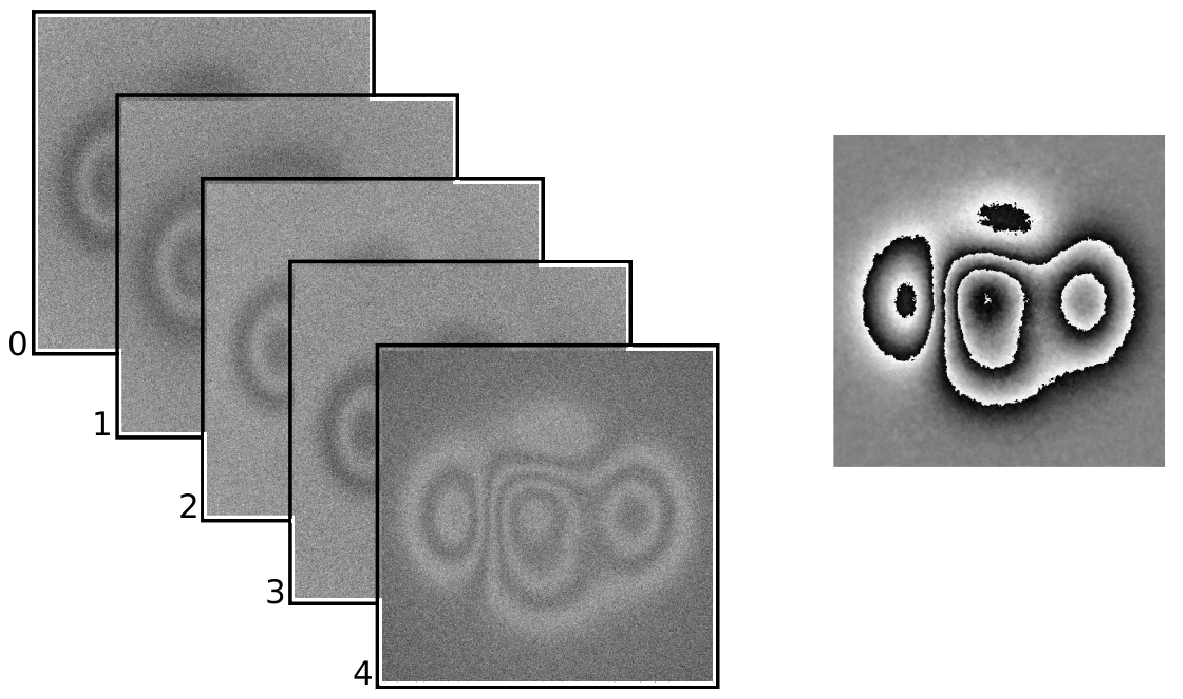
\includegraphics[scale=0.25]{Images/FaseSelfTuning.png}

\end{frame}
%%%%%%%%%%%%%%%%%%%%%%%%%%%% 25
\begin{frame}{Algoritmo auto-entonable para PSI}

Pasos calculados:
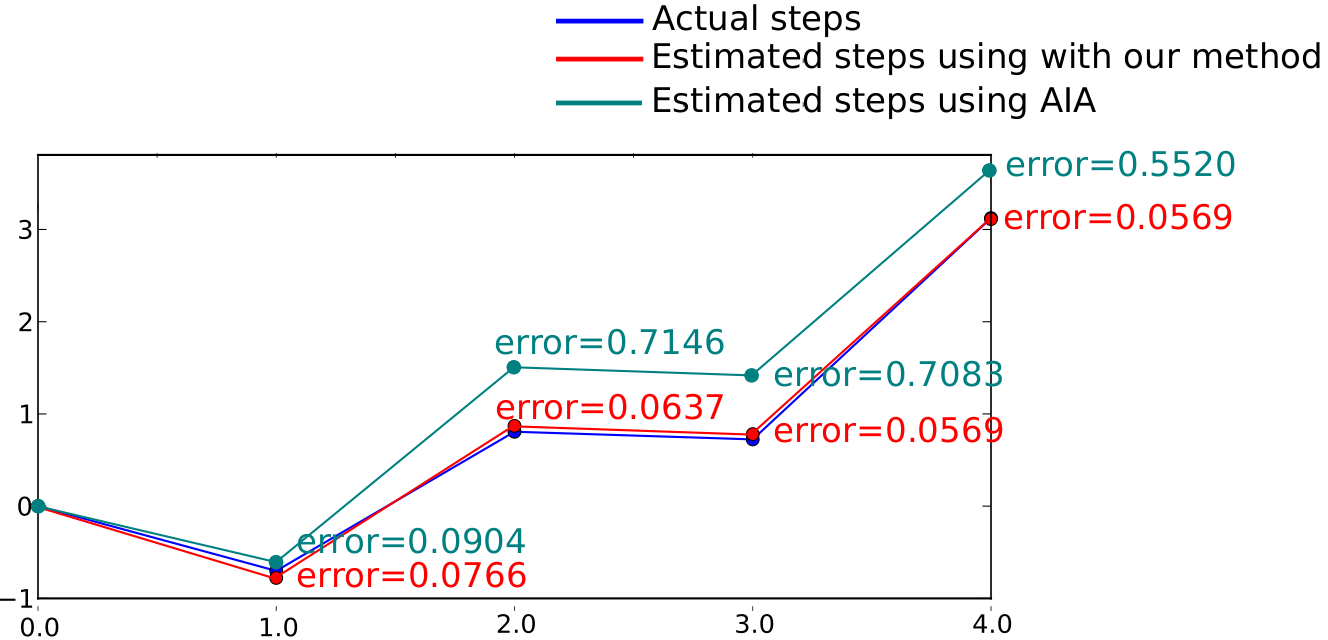
\includegraphics[scale=0.25]{Images/Self-tuningGraphError.png}

\end{frame}
%%%%%%%%%%%%%%%%%%%%%%%%%%%% 26
\begin{frame}{Algoritmo auto-entonable para PSI}

Conclusiones:
\begin{itemize}
     \item Este m\'etodo es robusto a pasos no constantes.
     \pause \item El m\'etodo es capaz de filtrar el ruido.
     \pause \item Recobra la fase y los pasos con error m\'inimo.
\end{itemize}

\end{frame}
%%%%%%%%%%%%%%%%%%%%%%%%%%%% 27
\begin{frame}{Algoritmo Adaptivo para PSI}

Interferograma con variaciones en cada punto:
\begin{center}
\begin{equation}
  I_k(x,y) = a(x,y)+b(x,y)cos[\phi_0(x,y) + \eta_k(x,y) + \omega_0 k],
\end{equation}

renombrando $\beta_k(x,y) = \eta_k(x,y) + \omega_0 k$
\begin{equation}
  I_k(x,y) = a(x,y)+b(x,y)cos[\phi_0(x,y) + \beta_k(x,y)]
\end{equation}

\end{center}
\end{frame}

%%%%%%%%%%%%%%%%%%%%%%%%%%%% 28
\begin{frame}{Algoritmo Adaptivo para PSI}

Suponiendo que conocemos las variaciones $\beta_k(x,y)$ podemos
calcular la $f(x,y)$:
\begin{center}

\begin{equation}
  U[a(x,y),f(x,y)]=\sum_{k=0}^{K-1}[a(x,y) + Re\{f(x,y) e^{i\beta_k (x,y)} \} -
I_k (x,y)]^2.
\end{equation}

\scriptsize{
\begin{multline*}
\left(\begin{array}{c}
a(x,y)\\
C(x,y)\\
S(x,y)
\end{array}\right) = \\
\left(\begin{array}{ccc}
K & \sum c_{k}(x,y) & \sum s_{k}(x,y)\\
\sum c_{k}(x,y) & \sum c_{k}(x,y)^{2} & \sum c_{k}(x,y)s_{k}(x,y)\\
\sum s_{k}(x,y) & \sum c_{k}(x,y)s_{k}(x,y) & \sum s_{k}(x,y)^{2}
\end{array}\right)^{-1}
\left(\begin{array}{c}
\sum I_{k}(x,y)\\
\sum I_{k}(x,y)C_{k}(x,y)\\
\sum I_{k}(x,y)S_{k}(x,y)
\end{array}\right)
\end{multline*}
}

\end{center}
\end{frame}
%%%%%%%%%%%%%%%%%%%%%%%%%%%% 29
\begin{frame}{Algoritmo Adaptivo para PSI}

Suponiendo que conocemos el campo complejo $f(x,y)$ podemos 
calcular $\beta_k$
\begin{center}

\begin{multline*}
U[a(x,y),g_{k}(x,y)]= \\ \sum_{m=0}^{M-1}\sum_{n=0}^{N-1}\Bigg[\{a(m,n)+Re\{g_{k}(m,
n)e^ { i\phi_{0}(x,y)}\}-I_{k}(m,n)\}h(x-m,y-n)\Bigg]^{2}
\end{multline*}
\footnotesize{
\begin{multline*}
\left(\begin{array}{c}
\hat{a}(x,y)\\
\hat{c}_{k}(x,y)\\
\hat{s}_{k}(x,y)
\end{array}\right)= \\ 
\left(\begin{array}{ccc}
[1s*h](x,y) & [\phi*h](x,y) & [\psi*h](x,y)\\{}
[\phi*h](x,y) & [\phi*h]^{2}(x,y) & [\phi\psi*h](x,y)\\{}
[\psi*h](x,y) & [\phi\psi*h](x,y) & [\psi*h]^{2}(x,y)
\end{array}\right)^{-1}
\left(\begin{array}{c}
[I_{k}*h](x,y)\\{}
[I_{k}\phi*h](x,y)\\{}
[I_{k}\psi*h](x,y)
\end{array}\right)
\end{multline*}
}

\end{center}
\end{frame}
%%%%%%%%%%%%%%%%%%%%%%%%%%%% 30
\begin{frame}{Algoritmo Adaptivo para PSI}

Fases experimentales obtenidas:
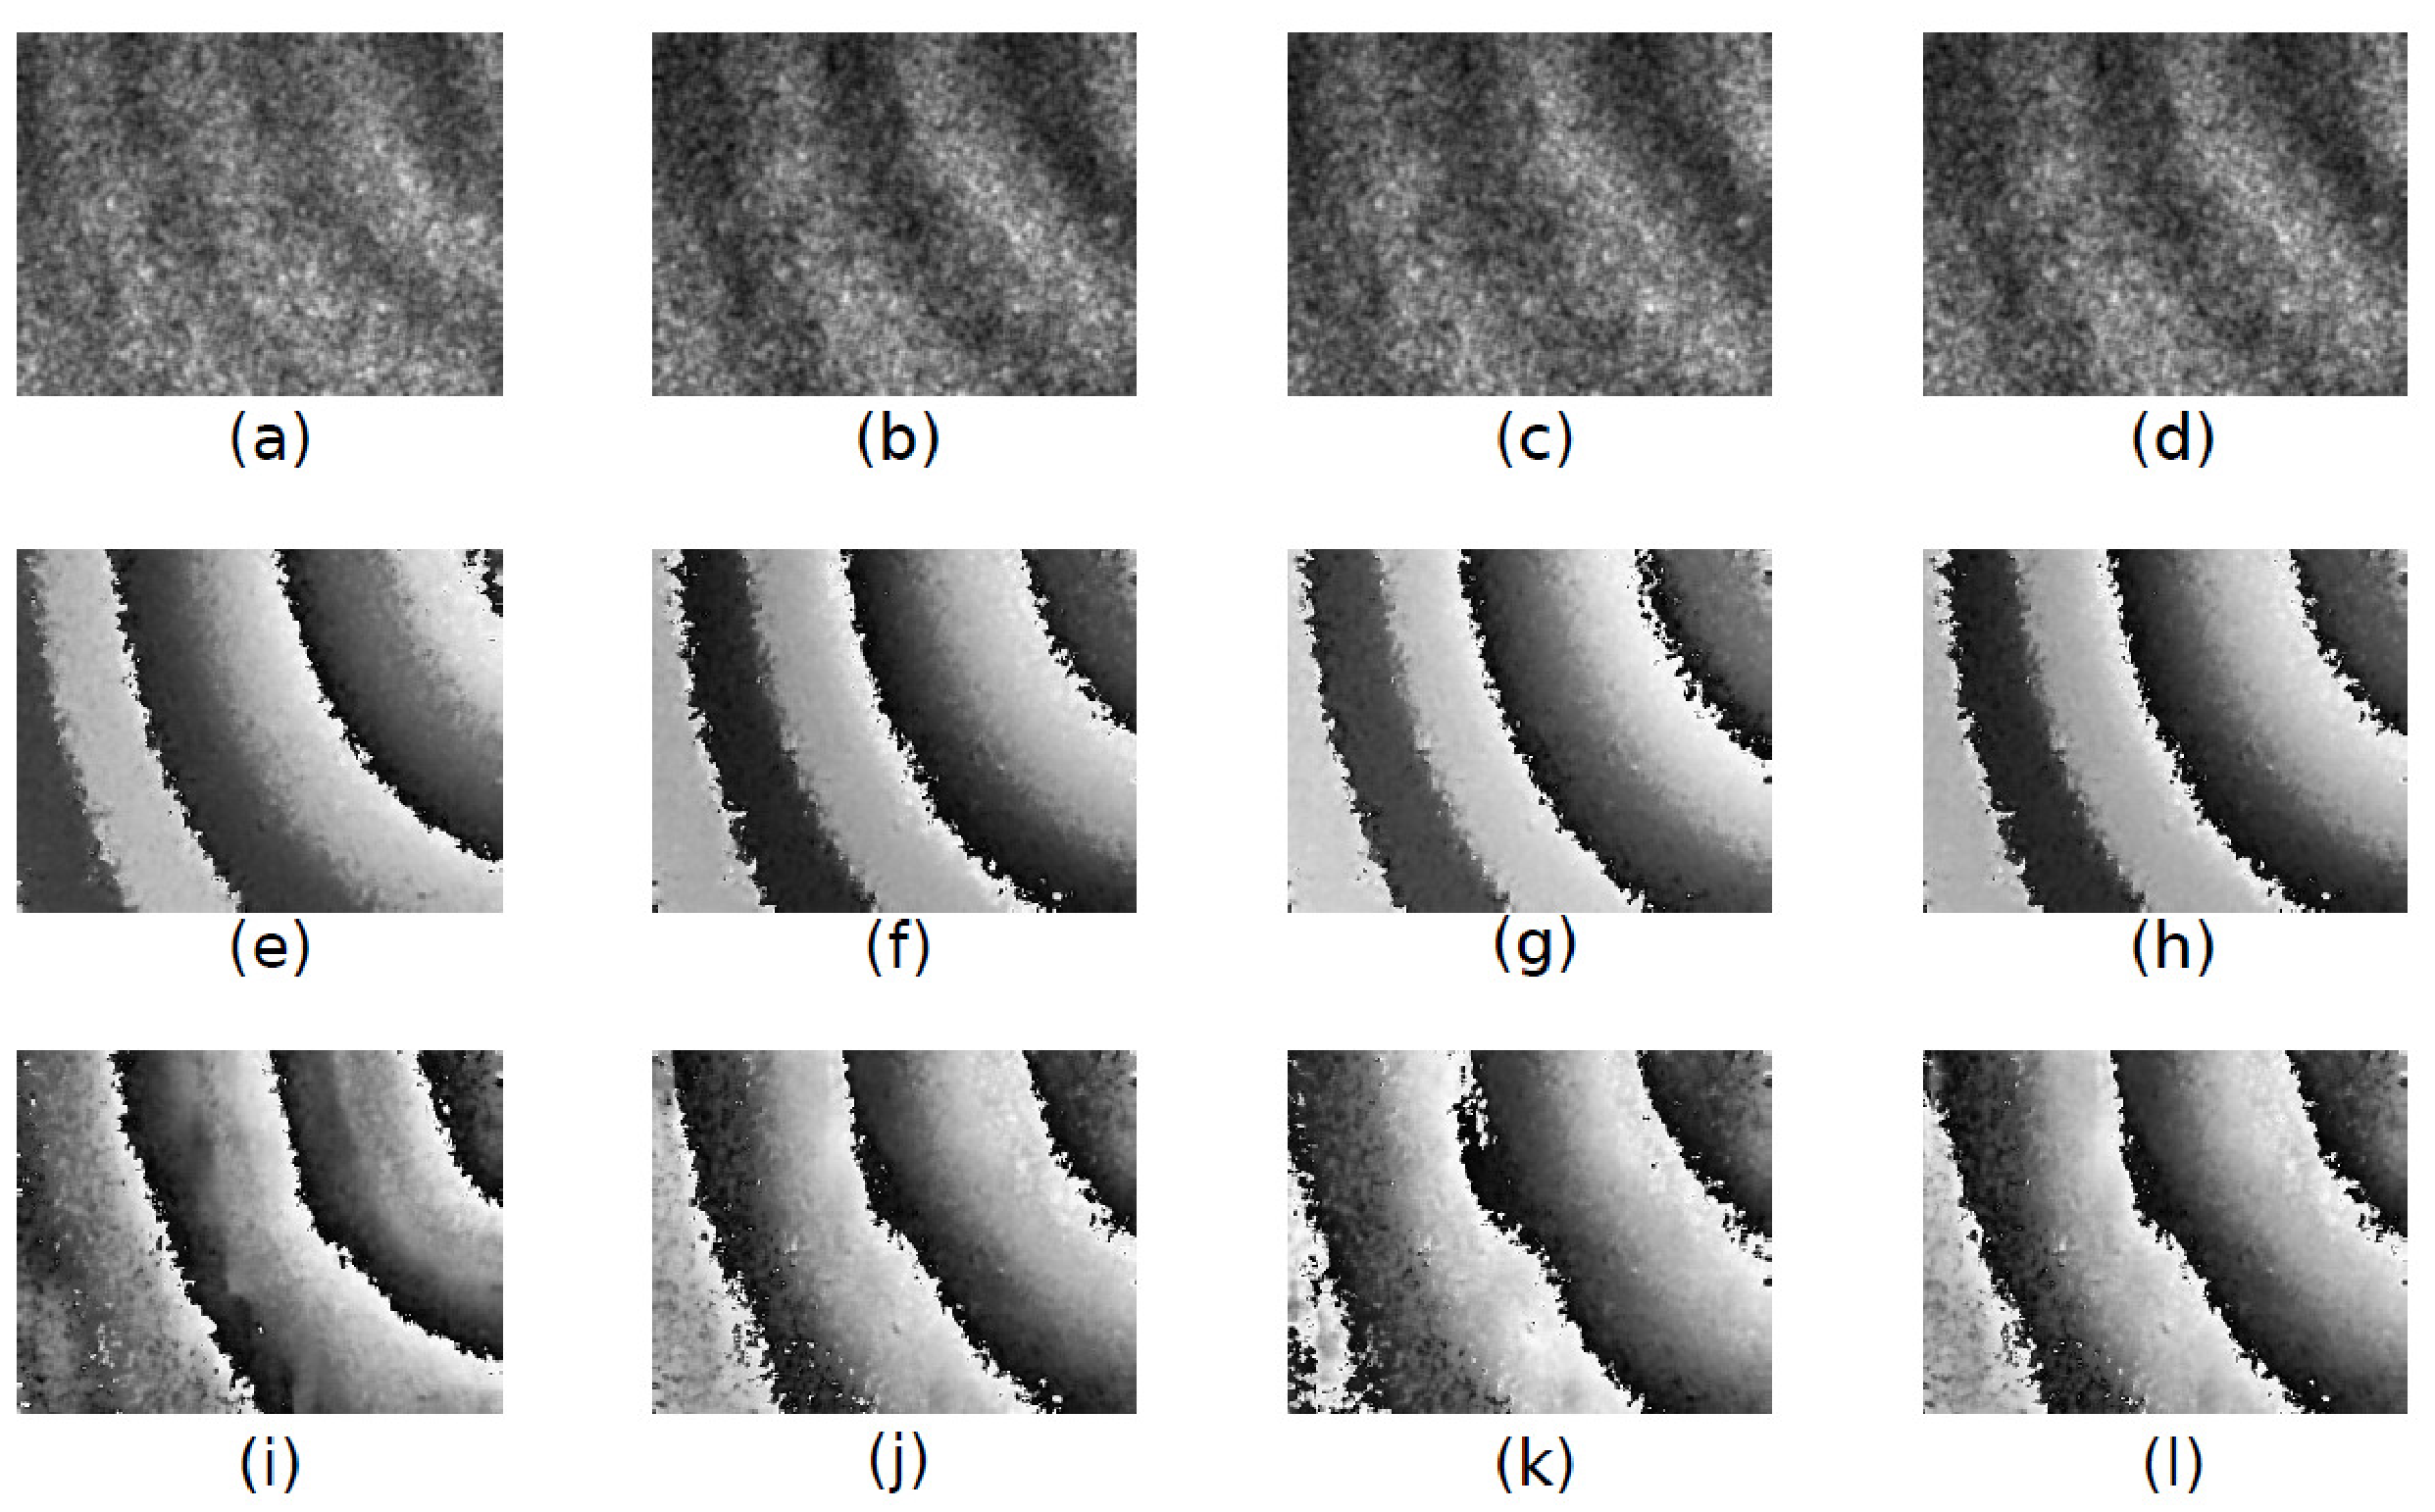
\includegraphics[scale=0.27]{Images/faseAdaptivePSI.pdf}

\end{frame}
%%%%%%%%%%%%%%%%%%%%%%%%%%%% 31
\begin{frame}{Algoritmo Adaptivo para PSI}

Conclusiones:
\begin{itemize}
     \item Este algoritmo no supone una fase est\'atica para cada punto.
     \pause \item El algoritmo calcula un desplazamiento para cada pixel.
     \pause \item El proceso es lineal y utiliza un estimador local pesado.
\end{itemize}

\end{frame}
%%%%%%%%%%%%%%%%%%%%%%%%%%%% 32
\begin{frame}{Corrector de fase  envuelta desentonada}

Funcional de energ\'ia:
\begin{center}
\begin{eqnarray*}
U(f) &=& \sum_{x,y\in L} \mid f(x,y) - g(x,y) \mid ^2 \nonumber\\
      &  &+ \lambda \sum_{x,y\in L} 
  \mid f(x,y) - f(x-1,y) e^{i u_{x,y}} \mid^2 \nonumber\\
  & & + \lambda \sum_{x,y\in L} \mid f(x,y) - f(x,y-1) e^{i v_{x,y}} \mid^2
\end{eqnarray*}
Para $g(x,y)= e^{i \phi^\varepsilon_{x,y}}$

\end{center}
\end{frame}
%%%%%%%%%%%%%%%%%%%%%%%%%%%% 33
\begin{frame}{Corrector de fase envuelta desentonada}
C\'alculo de las frecuencias espaciales en $x$:
\begin{center}

\begin{equation*}
  \nabla \phi_{x,y} = \nabla \left[ \arctan \left(\frac{\sin{\phi_{x,y}}}	
      {\cos{\phi_{x,y}}}\right)\right]
\end{equation*}

\begin{eqnarray*}
  u_{x,y} = \frac{\sin \phi \frac{\partial}{\partial x}  \cos \phi - \cos 
  \phi \frac{\partial}{\partial x} \sin \phi}{ \cos^2 \phi + \sin^2 \phi }
\end{eqnarray*}

\begin{equation*}
  \frac{\partial}{\partial x} \cos\phi_{x,y} = 
  \cos\phi_{x,y}-\cos\phi_{x+1,y},
\end{equation*}

\end{center}
\end{frame}
%%%%%%%%%%%%%%%%%%%%%%%%%%%% 34
\begin{frame}{Corrector de fase envuelta desentonada}
C\'alculo de las frecuencias espaciales en $y$:
\begin{center}

\begin{equation*}
  \nabla \phi_{x,y} = \nabla \left[ \arctan \left(\frac{\sin{\phi_{x,y}}}	
      {\cos{\phi_{x,y}}}\right)\right]
\end{equation*}

\begin{eqnarray*}
  u_{x,y} = \frac{\sin \phi \frac{\partial}{\partial x}  \cos \phi - \cos 
  \phi \frac{\partial}{\partial x} \sin \phi}{ \cos^2 \phi + \sin^2 \phi }
\end{eqnarray*}

\begin{equation*}
  \frac{\partial}{\partial y} \sin\phi_{x,y} = 
  \sin\phi_{x,y}-\sin\phi_{x,y+1}.
\end{equation*}

\end{center}
\end{frame}
%%%%%%%%%%%%%%%%%%%%%%%%%%%% 35
\begin{frame}{Corrector de fase envuelta desentonada}
Secuencia del mejoramiento de las frecuencias espaciales
\begin{center}

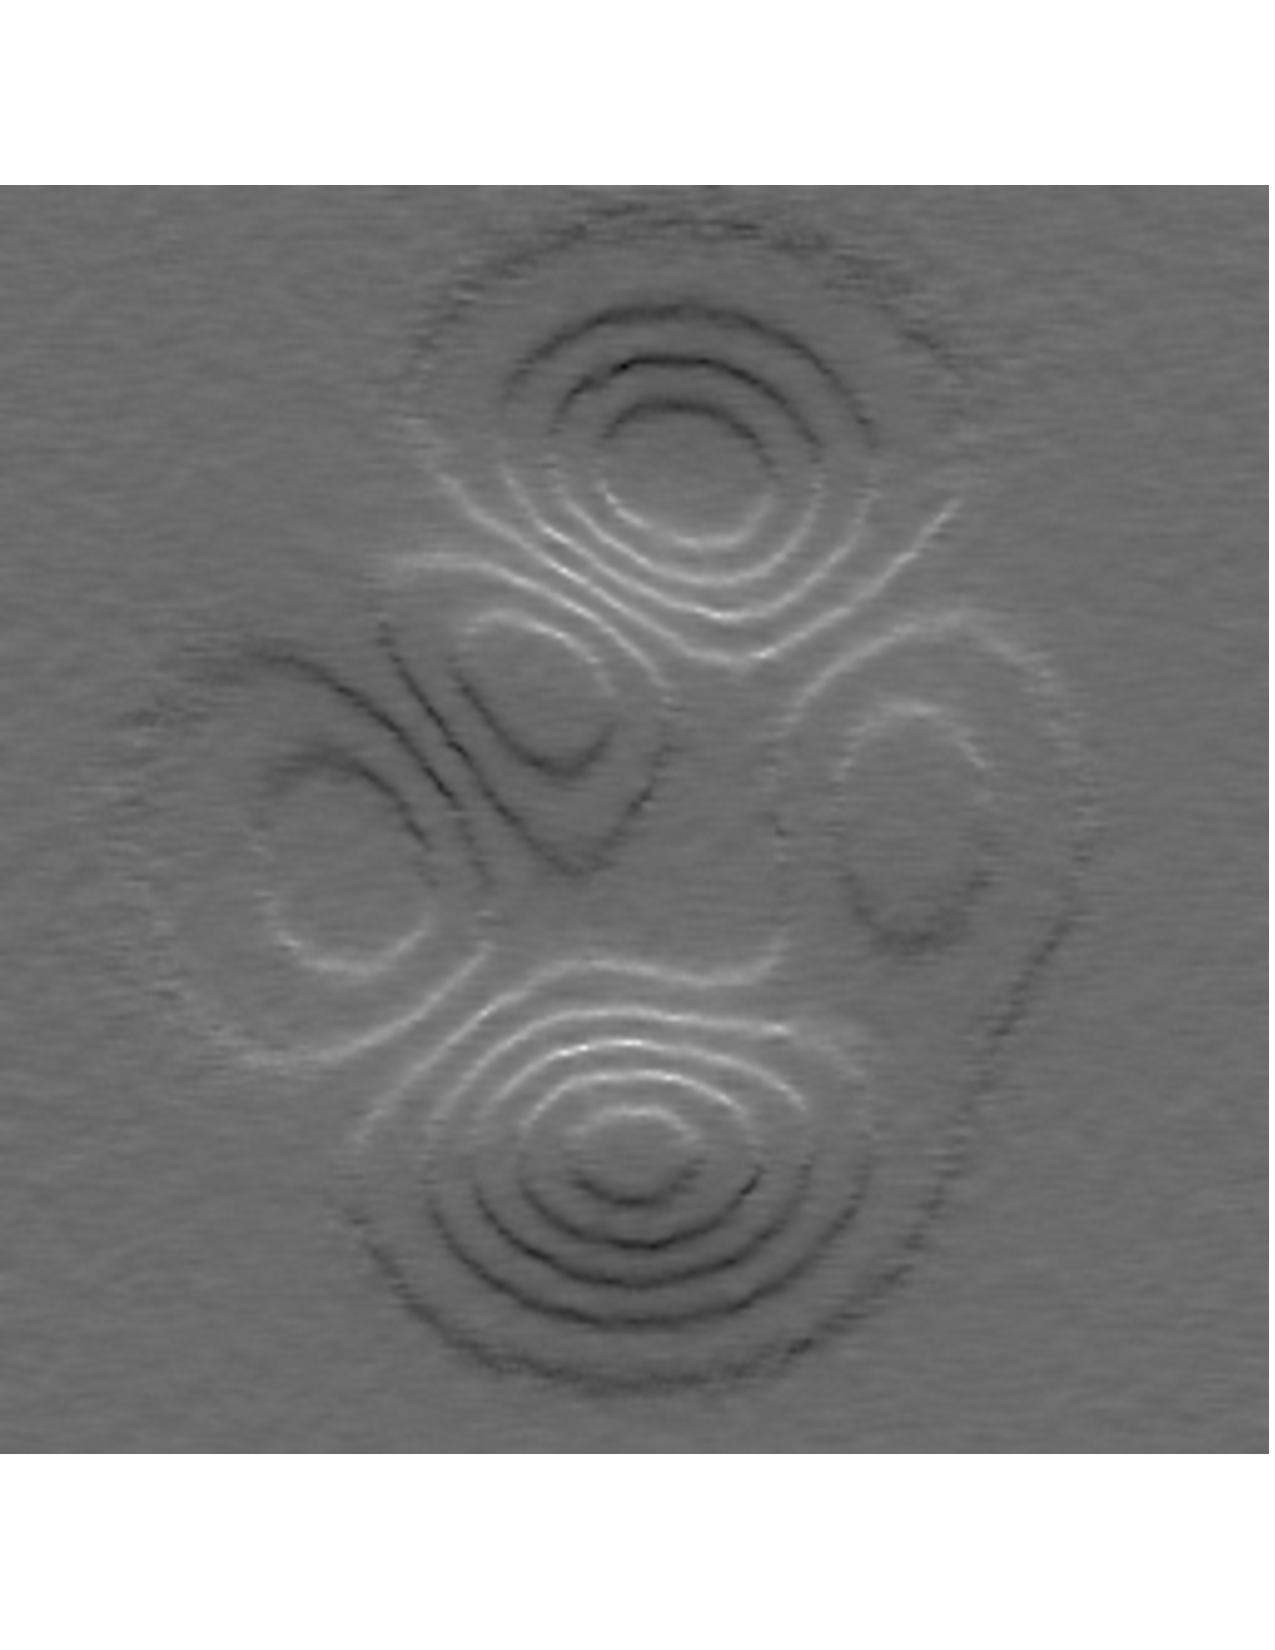
\includegraphics[scale=0.15]{Images/Fig_frecuencias1.pdf} \quad
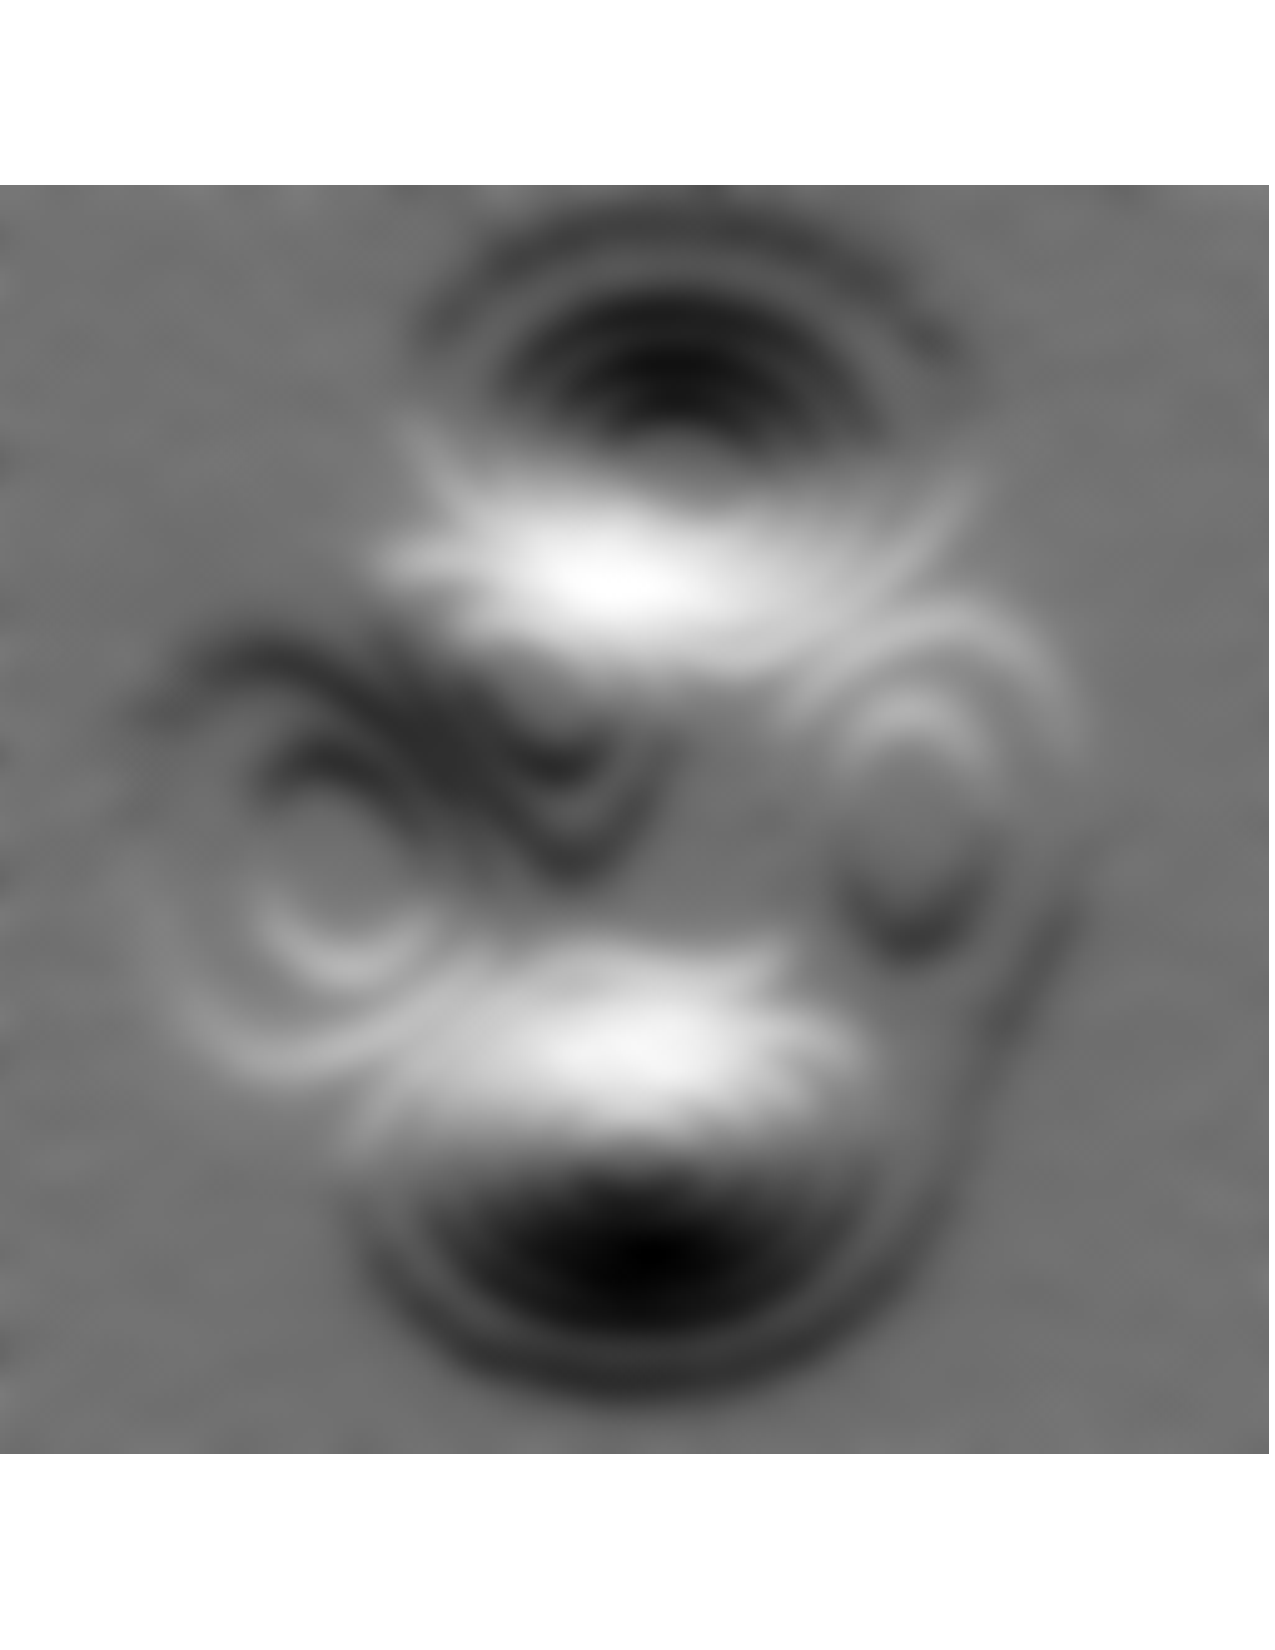
\includegraphics[scale=0.15]{Images/Fig_frecuencias2.pdf}\quad
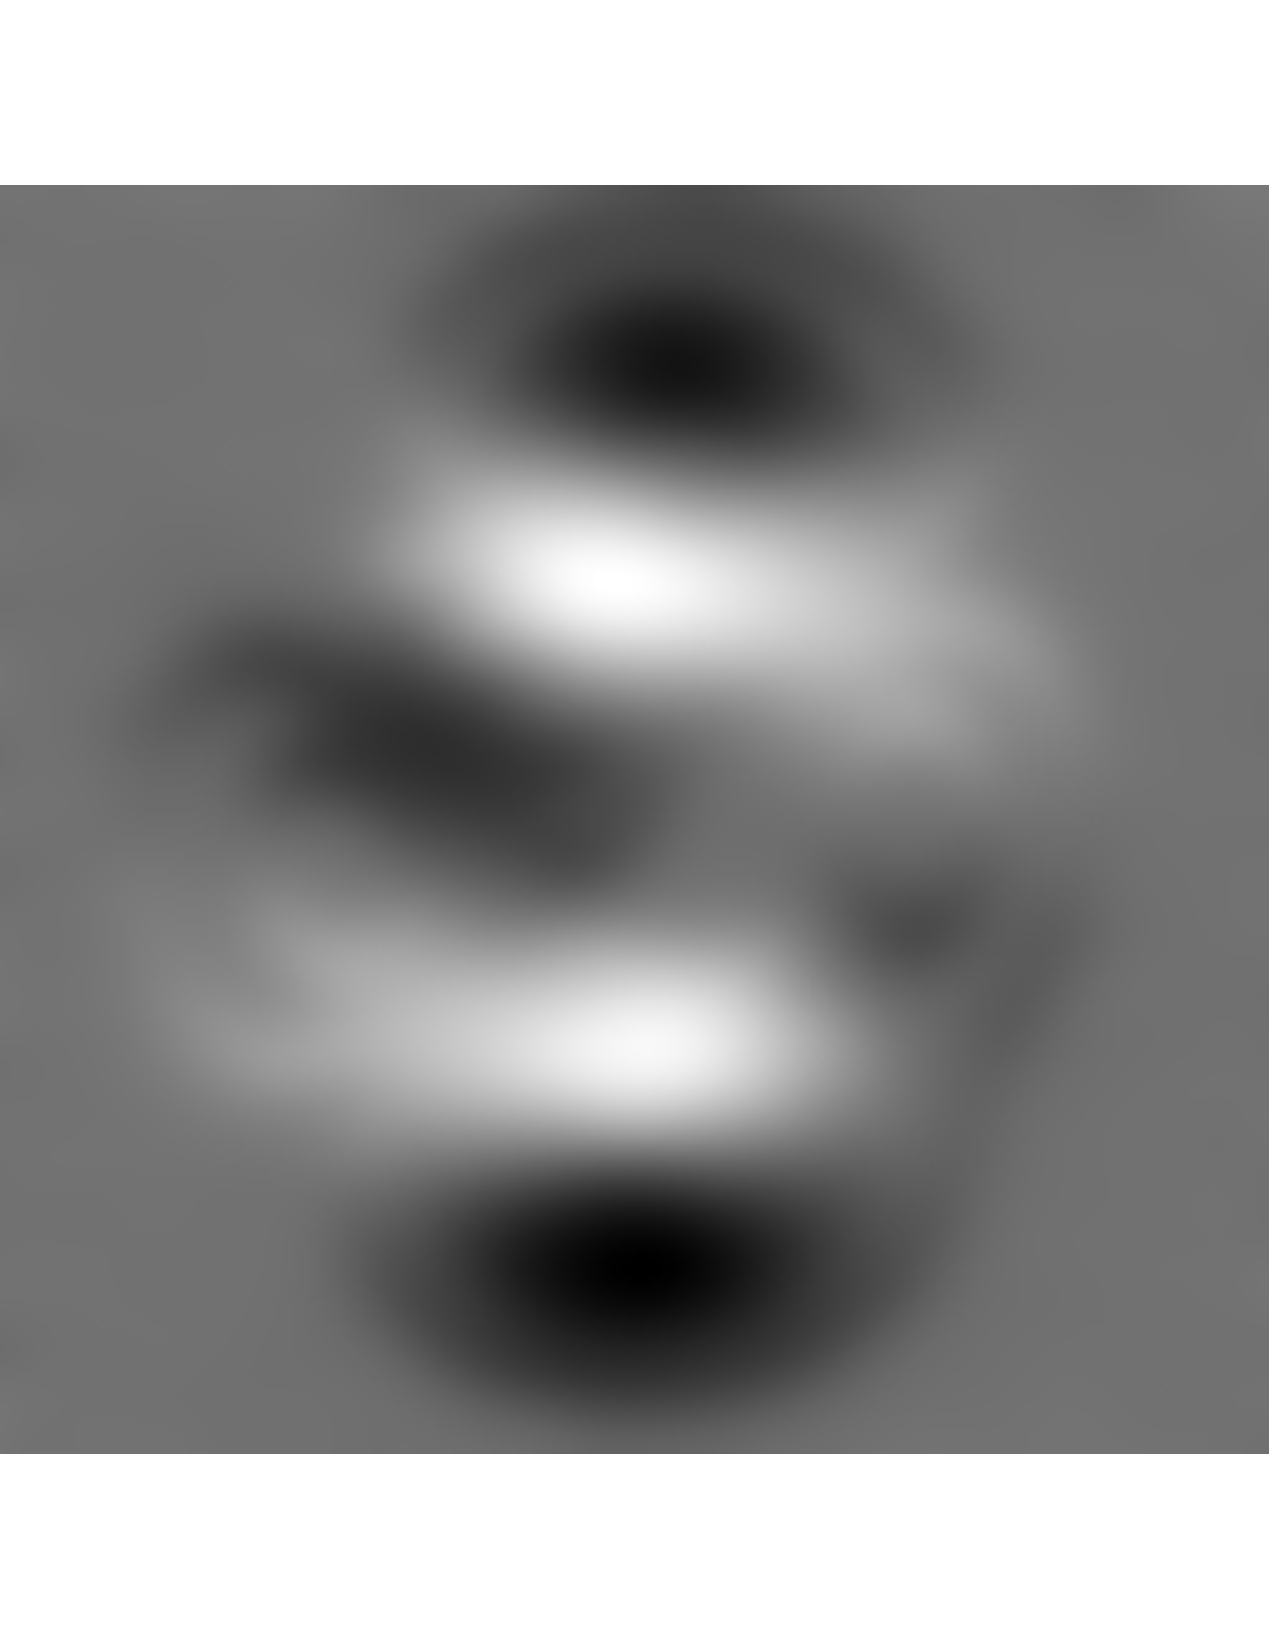
\includegraphics[scale=0.15]{Images/Fig_frecuencias3.pdf}


\end{center}
\end{frame}
%%%%%%%%%%%%%%%%%%%%%%%%%%%% 36
\begin{frame}{Corrector de fase envuelta desentonada}
Ejemplo de la fase envuelta mejorada
\begin{center}

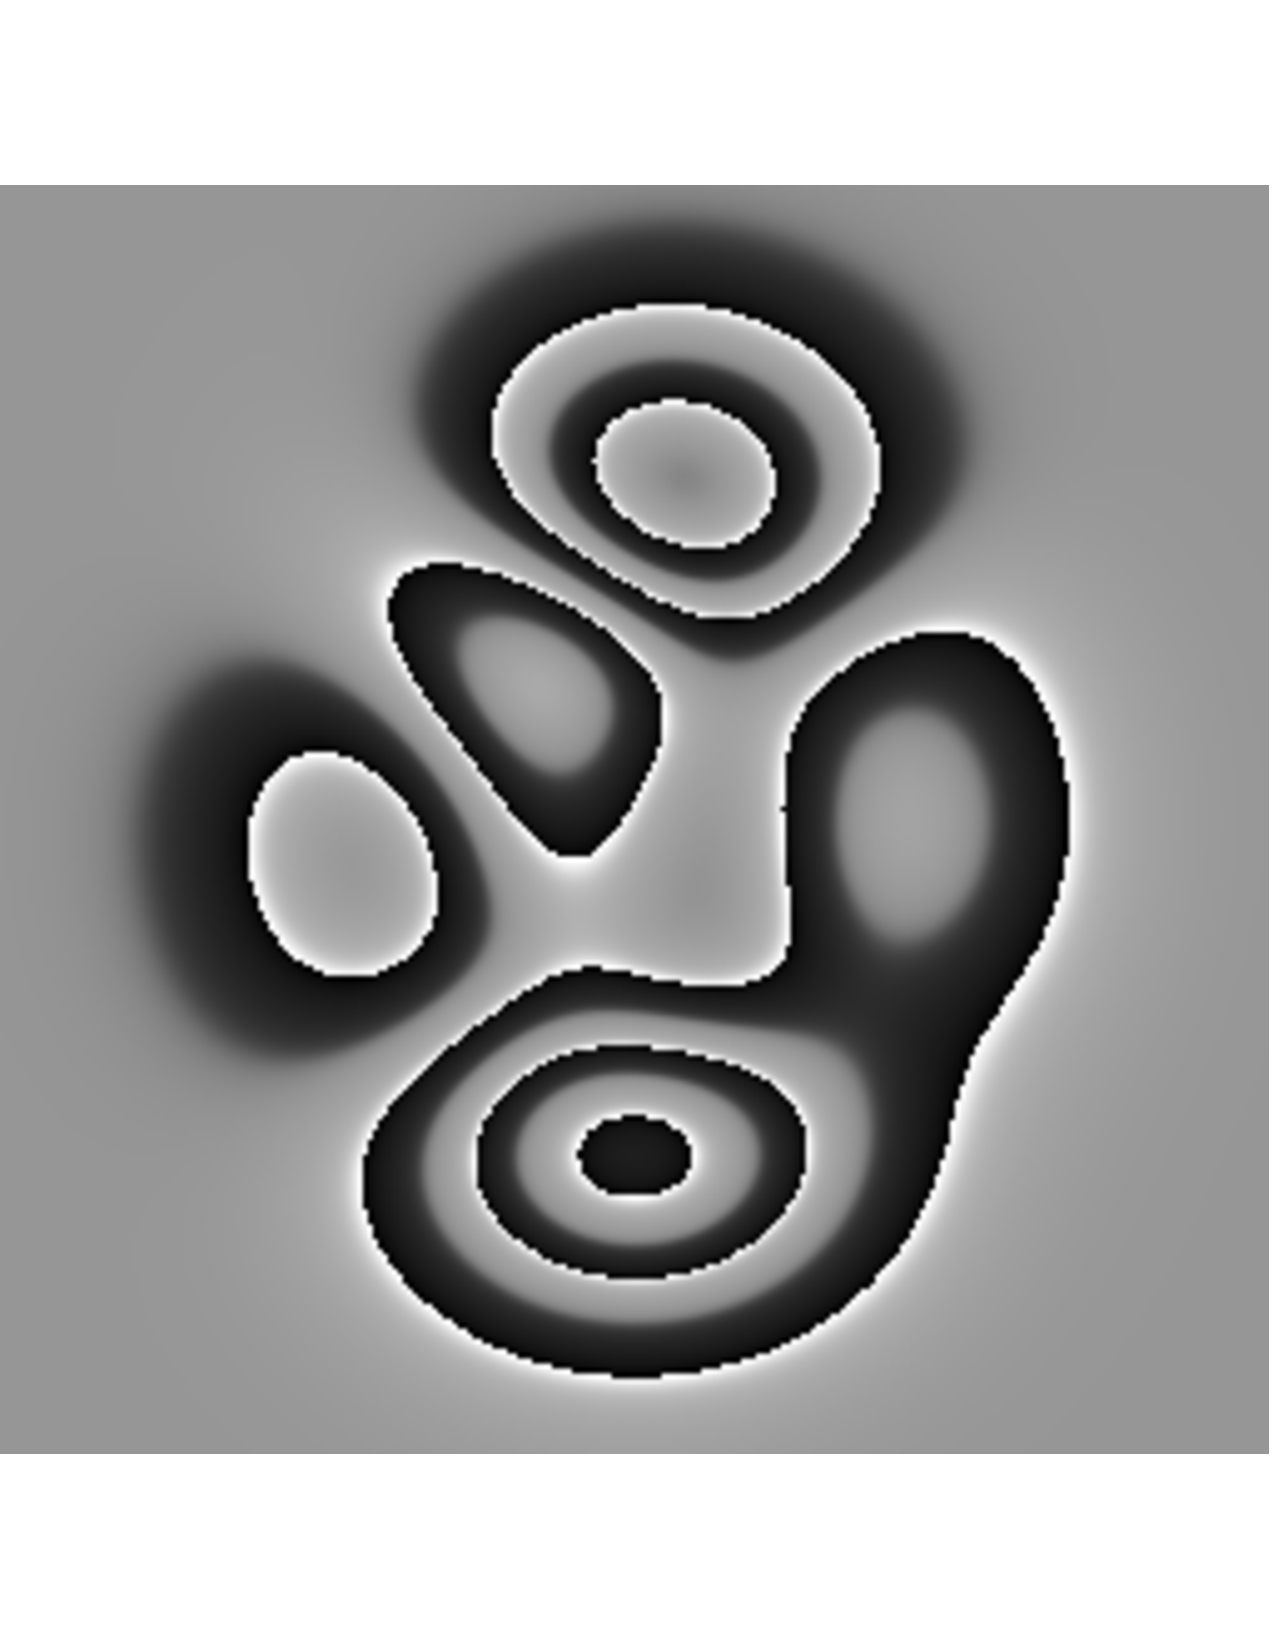
\includegraphics[scale=0.2]{Images/wfaseIdeal_error.pdf} \quad
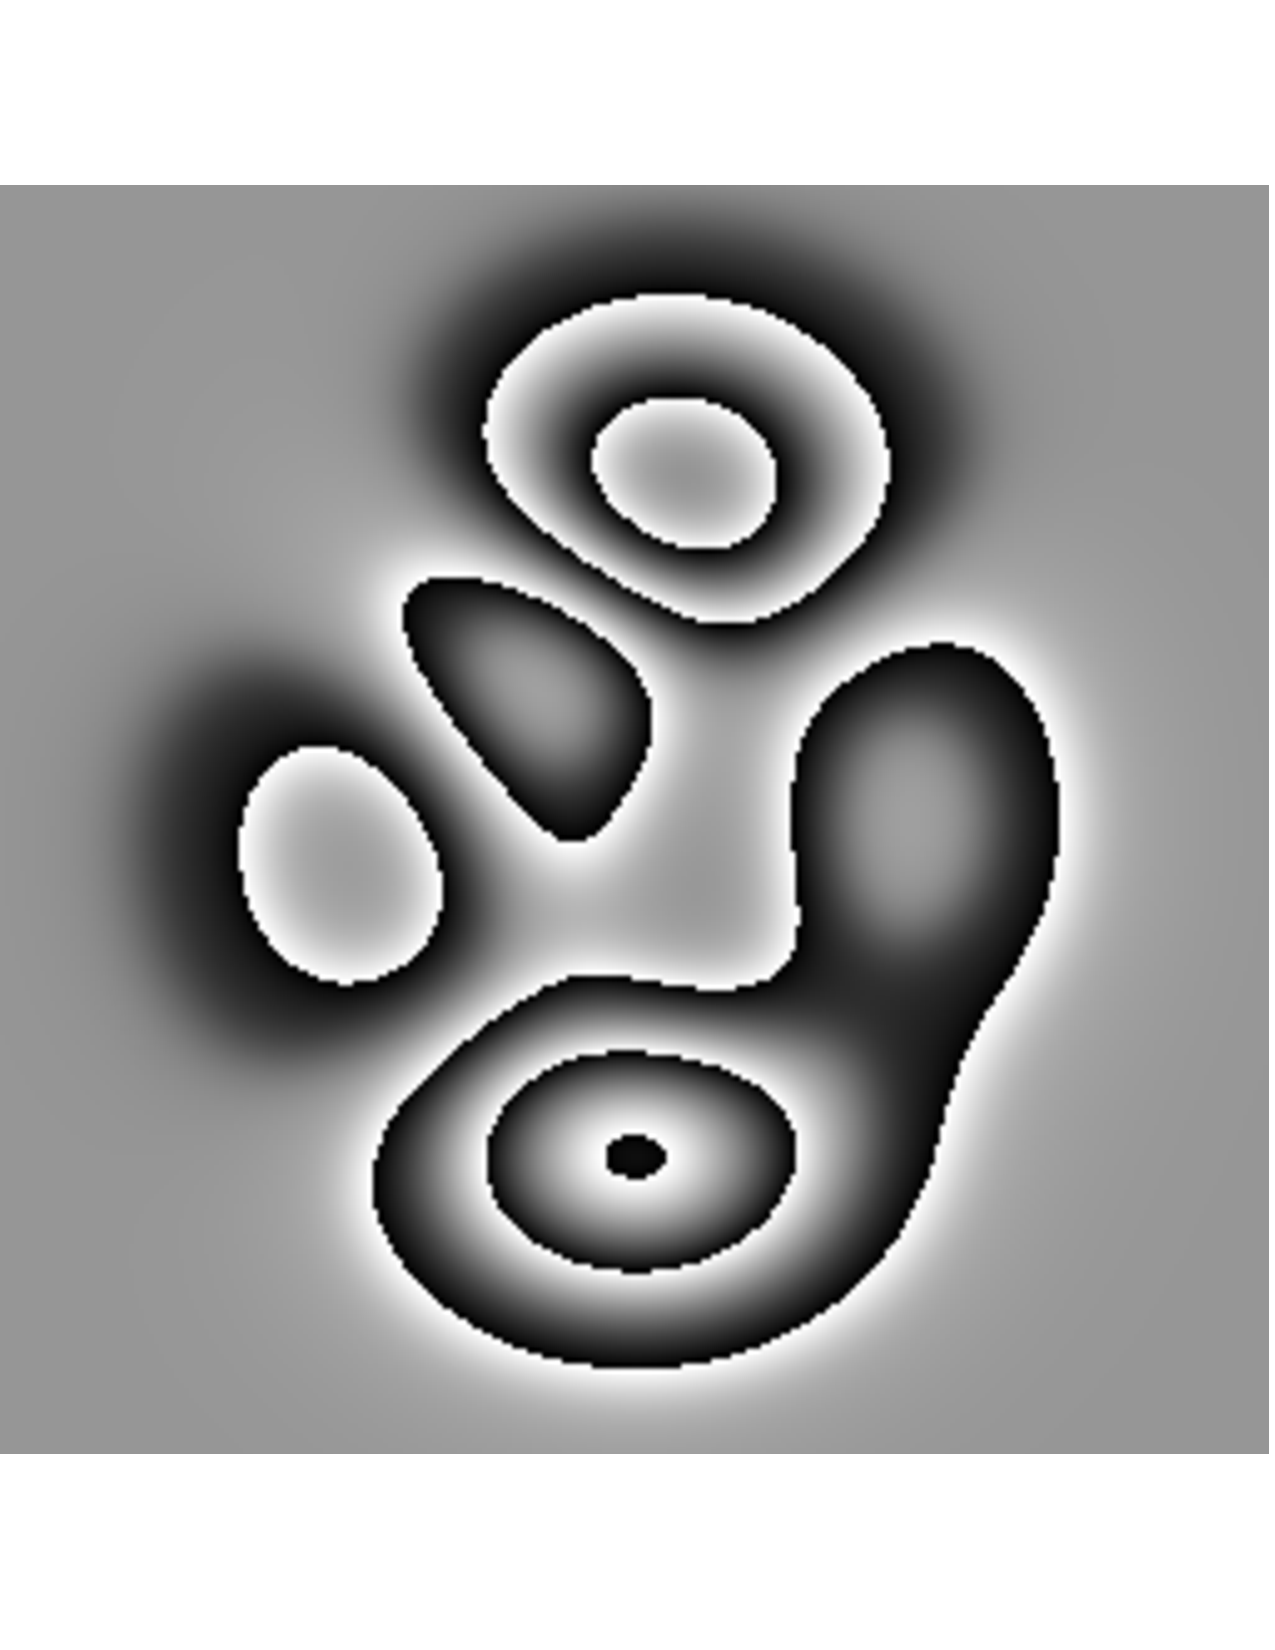
\includegraphics[scale=0.2]{Images/wfaseIdeal_mejorada.pdf}

\end{center}
\end{frame}
%%%%%%%%%%%%%%%%%%%%%%%%%%%% 37
\begin{frame}{Corrector de fase envuelta desentonada}
Ejemplo de la fase envuelta mejorada en 3D
\begin{center}

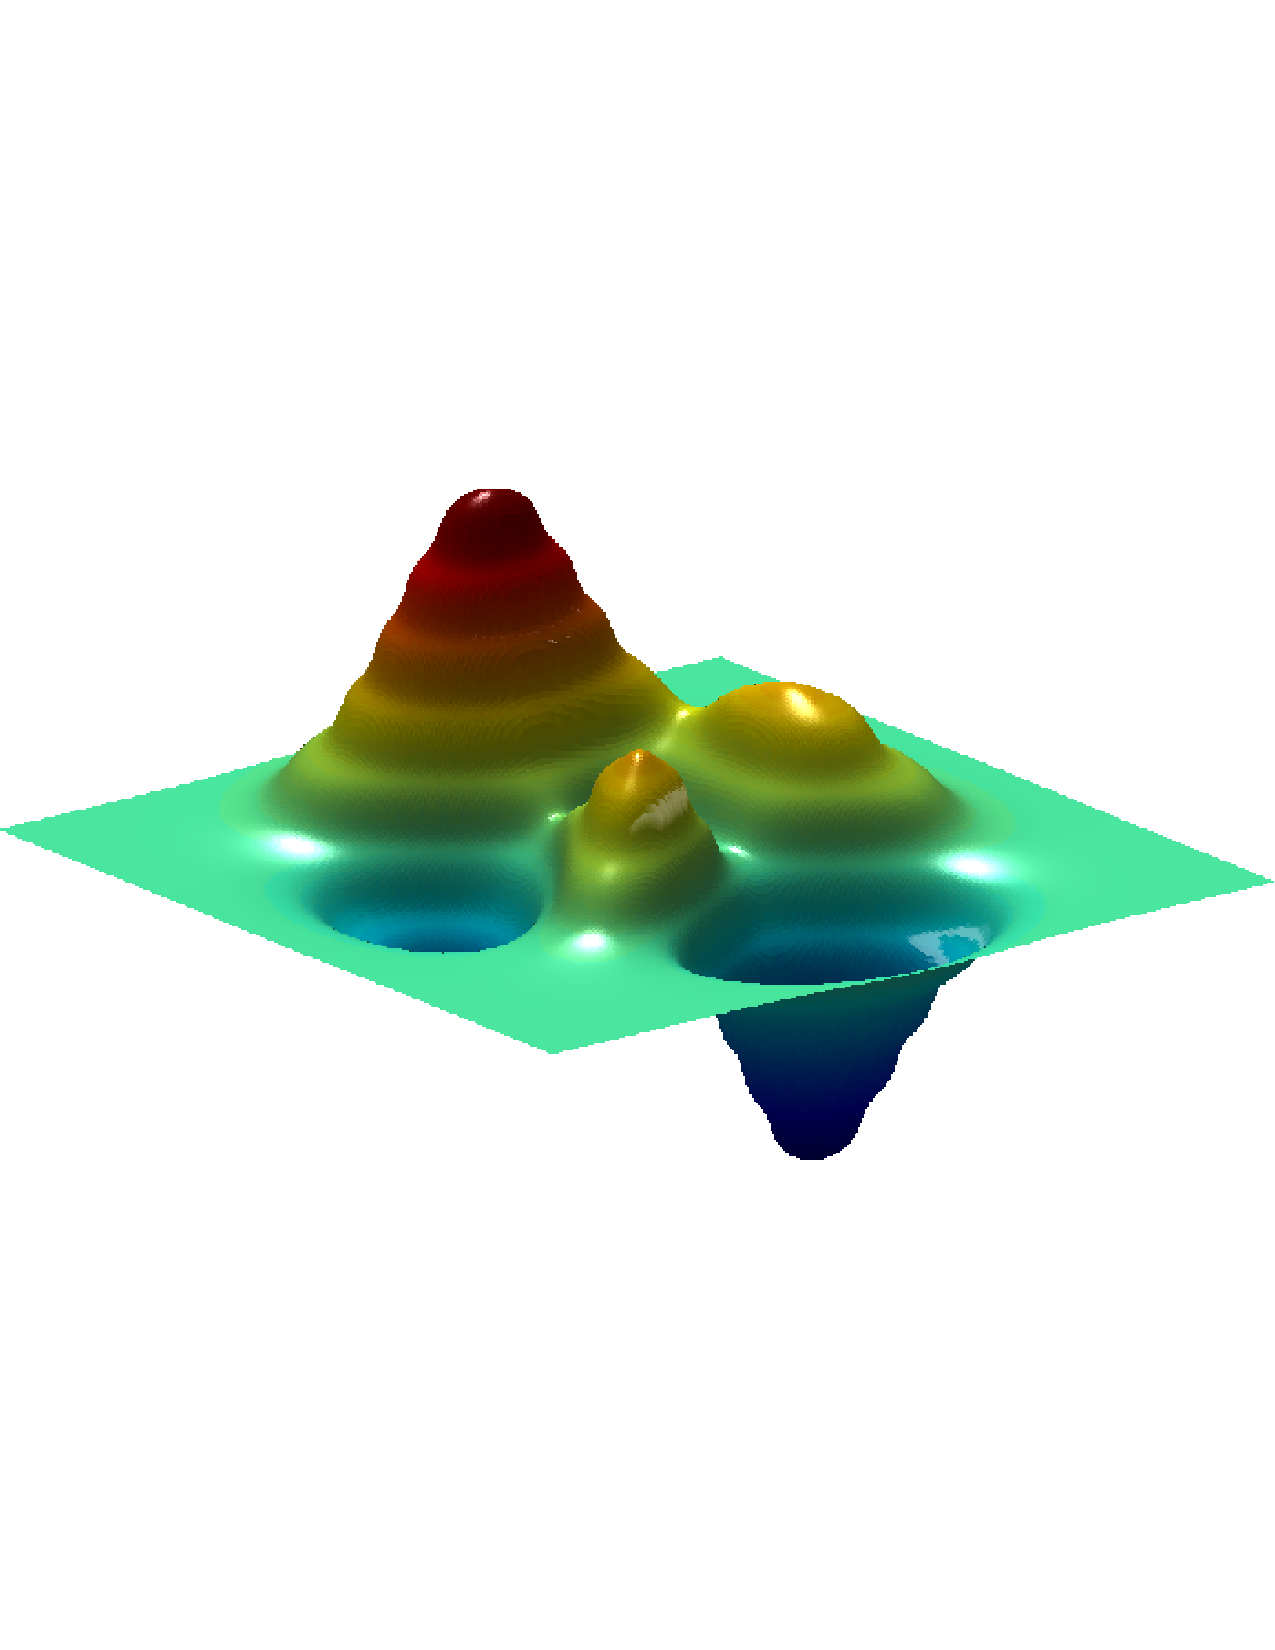
\includegraphics[scale=0.27]{Images/FaseError_Ideal_3D.pdf}
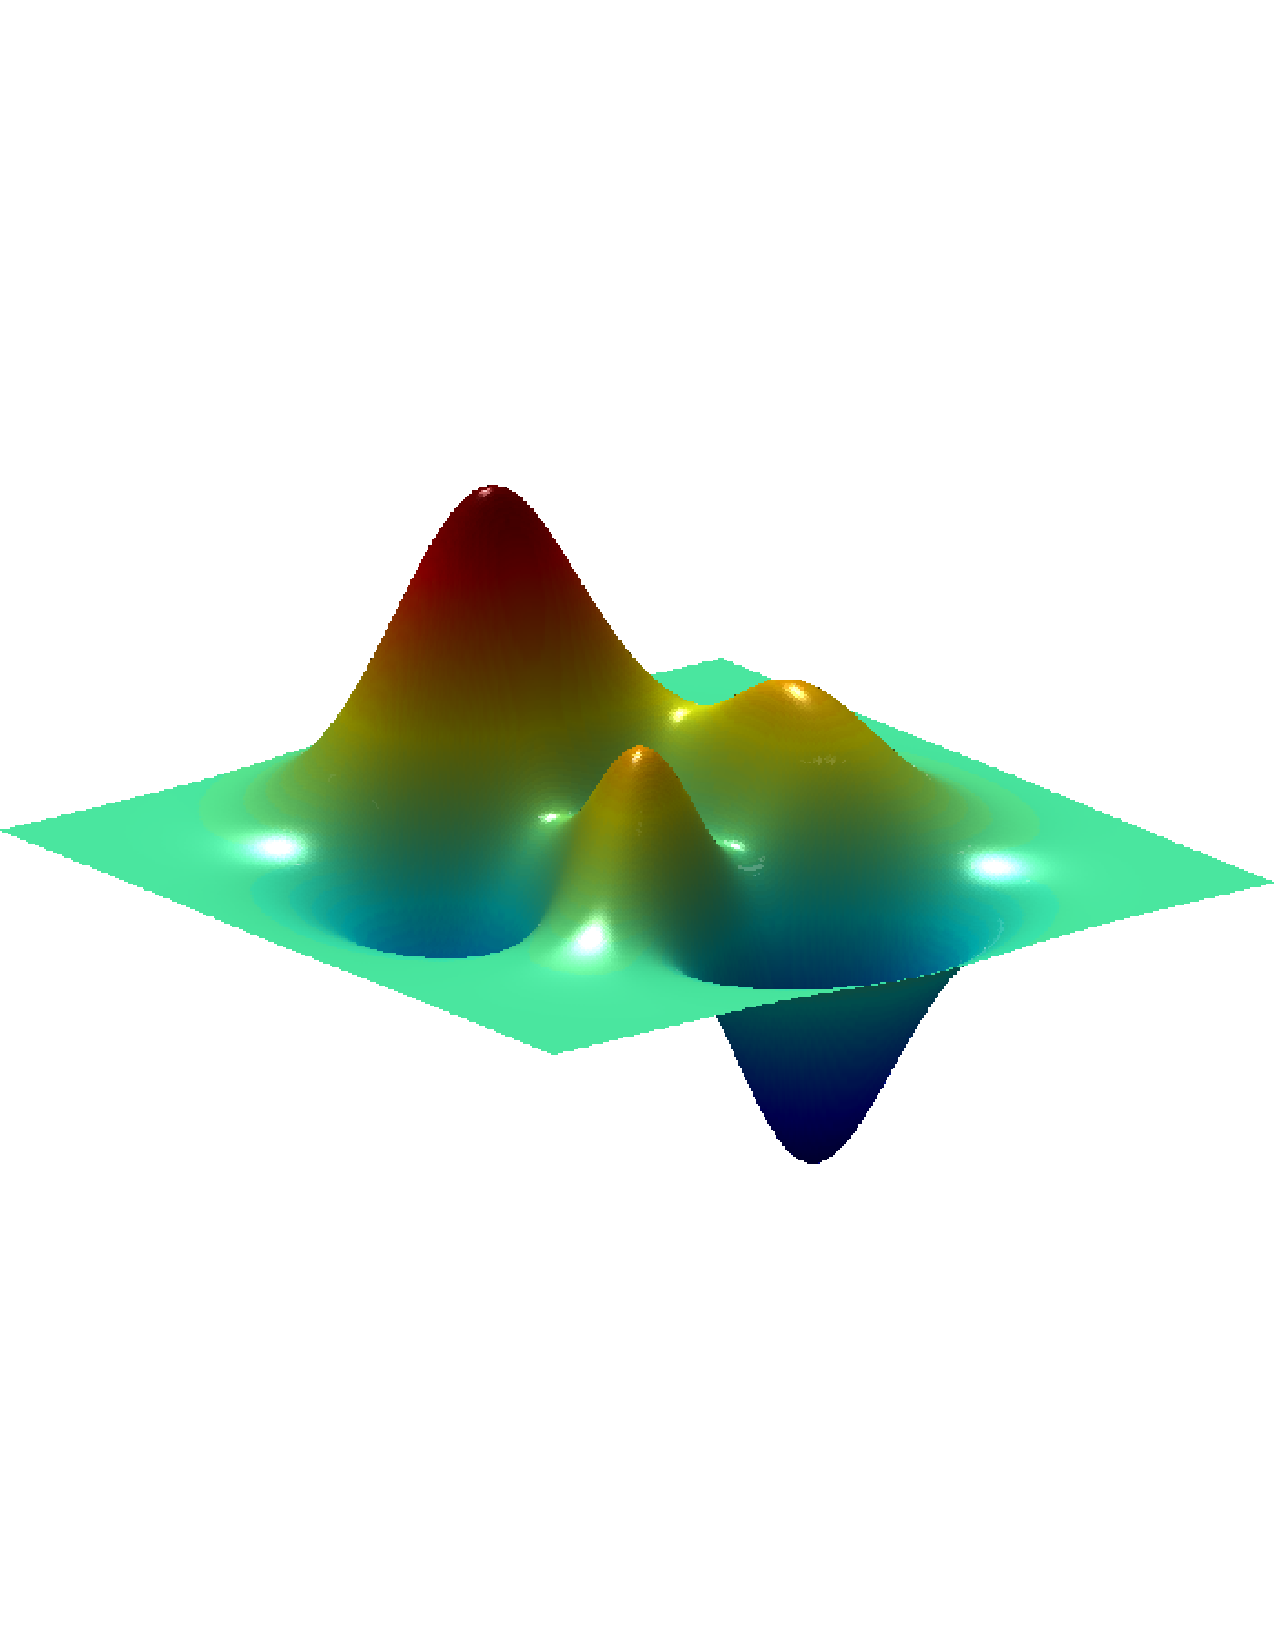
\includegraphics[scale=0.27]{Images/Fase_Ideal_3D.pdf}

\end{center}
\end{frame}
%%%%%%%%%%%%%%%%%%%%%%%%%%%% 38
\begin{frame}{Corrector de fase envuelta desentonada}
Conclusiones:
\begin{itemize}

\item El algoritmo es capaz de reducir el desentonamiento en la
  fase envuelta introducido por el algoritmo de cuadratura.

\pause \item El algoritmo es capaz de limpiar una fase envuelta
ruidosa sin perder informaci\'on por el filtrado.

\pause \item La estrategia de remover el desentonamiento de la fase
envuelta es una aproximaci\'on nunca antes propuesta.

\pause \item El algoritmo es lineal y por ende estable.

\end{itemize}
\end{frame}
%%%%%%%%%%%%%%%%%%%%%%%%%%%% 39
\begin{frame}{Producci\'on cientifica}

\begin{itemize}
\small{
            \item  \textbf{Medina O}, Estrada JC. "Full-field two-dimensional 
              least-squares method for phase-shifting interferometry".
              Opt. Eng. 0001;53(11):114106.
            \item \textbf{Orlando Medina}; Julio C. Estrada; Manuel Servin. 
              “Regularized least-squares algorithm for phase-shifting 
              interferometry” MOPM 4-6 sep 2013.
            \item \textbf{Orlando Medina}; Julio C. Estrada; Manuel Servin. 
              “Regularized self-tuning phase demodulation for
              phase-shifting interferometry with arbitrary phase
              shifts” Proc. SPIE 8493, Interferometry XVI: 
              Techniques and Analysis, 84930K (September 13, 2012);
            \item M. Servin, J.C. Estrada and \textbf{Orlando Medina}. 
              “Fourier transform demodulation of pixelated phase-mask
              interferograms” Optics Express, Vol. 18, Issue 15,
              pp. 16090-16095 (2010).
              \item \textbf{Orlando Medina}; Julio C. Estrada; Manuel Servin,
                “Demodulación temporal de interferogramas” VII
                Simposio La \'Optica en la Industria. 10-12 sep 2009.
              \item Nombramiento de \textbf{Candidato en el SNI}.
}
\end{itemize}
\end{frame}
%%%%%%%%%%%%%%%%%%%%%%%%%%%%
\end{document}